
\documentclass[12pt]{article}


\usepackage{cite}
\usepackage{graphicx}
\usepackage{subfigure}
\usepackage{epsfig}
\usepackage{epstopdf}
\usepackage{subfigure}
\usepackage{calc}
\usepackage{amssymb}
\usepackage{amstext}
\usepackage[fleqn]{amsmath}


\title{VelaLab reference Manual}

%\author{
%        Vitaly Surazhsky \\
%                Department of Computer Science\\
%        Technion---Israel Institute of Technology\\
%        Technion City, Haifa 32000, \underline{Israel}
%            \and
%        Yossi Gil\\
%        Department of Computer Science\\
%        Technion---Israel Institute of Technology\\
%        Technion City, Haifa 32000, \underline{Israel}
%}

\date{\today}


\begin{document}
\maketitle

%\begin{abstract}
%This is the paper's abstract \ldots
%\end{abstract}



\section{System Architecture}


\begin{figure}[h]
	\centering
	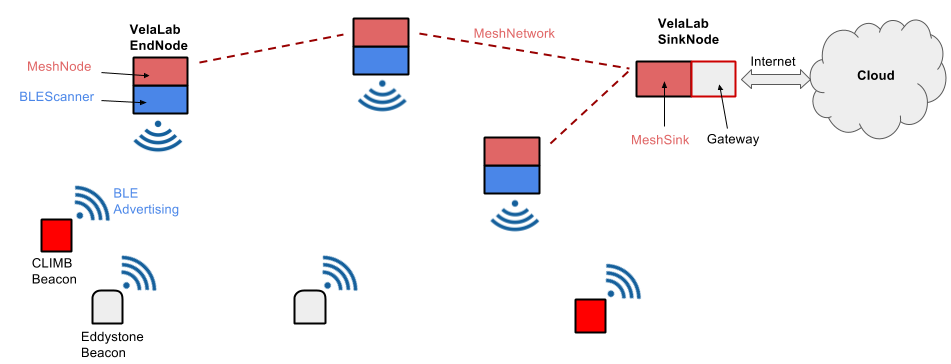
\includegraphics[width=0.98\columnwidth]{fig/Architecture.png}
	\caption{}
	\label{fig:system}
\end{figure}



\subsection{Namings and definitions}

%\subsubsection{BLE\_Beacon}
\textbf{BLE\_Beacon}

Any beacon device that can be detected from the system. Now it can be of two types: \textit{CLIMB\_Beacon} and  \textit{Eddystone\_Beacon}.
\\

\noindent \textbf{VelaLab\_EndNode}

One of the nodes forming the BLE+mesh network. It is formed by a \textit{BLE\_Scanner} and a \textit{Mesh\_Node}, which communicate via a serial connection (UART).


\noindent \textbf{BLE\_Scanner}

BLE part of an EndNode, based on the Nordinc nRFxx and implemented on the nRFxxx development board.
\\

\noindent \textbf{Mesh\_Node}

Mesh/Contiki part of an EndNode, based on the TI CCxxxxx and implemented on the Lauchpad xxx dev board.
\\

\noindent \textbf{VelaLab\_SinkNode}

The sink/gateway node of the network. It combines the Mesh\_Sink and the Gateway, which are connected using the serial to USB feature on the Mesh\_Sink. It does not have the BLE\_Scanner (only mesh and gateway)
\\

\noindent \textbf{Mesh\_Sink}

The sink node for the mesh/contiki network. Its hardware is equivalent to a Mesh\_Node, but it has a different firmware.
\\

\noindent \textbf{Gateway}

The gateway between the network and the internet/cloud. It is implemented using a Raspberry PI 3 (RPI). The Mesh\_Sink is connected through a USB port and it connects to the internet through Ethernet or WiFi.
\\

\noindent \textbf{Contact\_Data Structure}

\textit{Contact\_Data} is the data structure containing the information about the contact of one BLE Beacon. A \textit{Report} is an array of \textit{Contact\_Data} containing all the data received during the last epoch. All the reported parameters refer to the last epoch.
\\

\begin{tabular}{l|l|l}
Field 		& Type 		& Size (Byte)\\
\hline
\texttt{NodeID} 		& uint		& 6\\
\texttt{lastRSSI} 		& int			& 1\\
\texttt{maxRSSI} 		& int			& 1\\
\texttt{pktCounter} 	& u8			& 1\\
\end{tabular}
\\

\noindent \textbf{Back-End Data Structure (as in CLIMB)}

Data structure containing the information to be sent from the gateway to the server, encoded as a json object. Each call send an array of such objects.
\\

\begin{tabular}{l|l}
Field 			& Type\\
\hline
\texttt{wsnNodeId} 		& string	 \\
\texttt{eventType} 		& int		 \\
\texttt{timestamp} 		& int		 \\
\texttt{payload} 			& object	 \\
\end{tabular}
\\

Payload may contain:
\\

\begin{tabular}{l|l}
Field 			& Type 	\\
\hline
\texttt{passengerId} 		& string	 \\
\texttt{latitude} 			& float	 \\
\texttt{longitude} 		& float	 \\
\texttt{accuracy} 			& float	 \\
\end{tabular}
\\

%[{
%    "wsnNodeId" : "<id>",
%    "eventType" : 901,
%    "timestamp" : <timestamp>,
%    "payload" : {
%        "passengerId" : "a511a089-ab7a-446f-a8c2-4c208d4425c5",
%        "latitude" : 46.0678106,
%        "longitude" : 11.1515548,
%        "accuracy" : 18.5380001068115
%    }
%}]


\section{Beacons}

Types:
\begin{itemize}
\item{CLIMB (custom)}
\item{Eddystone}
\end{itemize}




\section{VelaLab End-Node}

Components:
\begin{itemize}
\item{BLE Scanner}
\item{Mesh Node}
\end{itemize}



\subsection{Hardware interconnection}

fig...

\begin{figure}[!h]
	\centering
	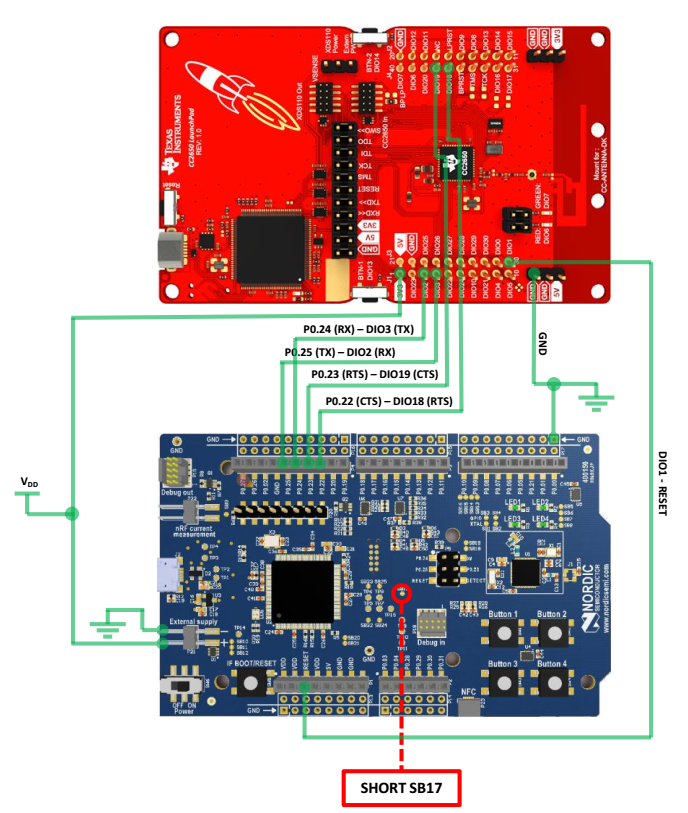
\includegraphics[width=0.7\columnwidth]{fig/VelaNode_hw.png}
	\caption{}
	\label{fig:system}
\end{figure}

The Launchpad image refers to the revision 1.0 of the hardware. In that version the DIO2 and DIO3 pins were incorrectly labelled (labels are swapped with respect to actual pin location). This scheme refers to the actual wiring position, then discard any label on the board and just wire as shown.


\subsection{Communication protocol}

UART communication protocol between BLE Scanner and Mesh Node


\section{VelaLab Sink-Node}

Components:
\begin{itemize}
\item{Mesh Sink}
\item{Gateway}
\end{itemize}

\subsection{Hardware interconnection}


Launchpad usb output to RPI's USB


\subsection{Communication protocol}


UART communication protocol between Mesh Sink and Gateway







%\bibliographystyle{abbrv}
%\bibliography{main}

\end{document}
This is never printed